% Revision summary (2026-04-08):
% - Reworked the document into an FYP-compliant dissertation package with title page,
%   abstract metadata, acknowledgements, table of contents, references before appendices,
%   and roman-to-arabic page numbering.
% - Reframed the thesis around the core empirical insight that statistical leadership and
%   economic signal leadership diverge in intraday IV-curve forecasting.
% - Strengthened the introduction, critical literature review, methodology, results
%   interpretation, and discussion so the document reads as one coherent study rather than
%   a stitched benchmark log.
% - Integrated the completed winner-versus-all-competitors appendix and block-bootstrap
%   significance analysis for the final retuned xLSTM benchmark, including the
%   attention-pooled LSTM and transformer controls.
% - Moved implementation architecture into the experimental-design chapter and added
%   appendices for dataset schema, benchmark configuration, and robustness notes.
\documentclass[12pt]{report}

\usepackage[a4paper,margin=1in]{geometry}
\usepackage[T1]{fontenc}
\usepackage[utf8]{inputenc}
\usepackage{lmodern}
\usepackage{microtype}
\usepackage{setspace}
\usepackage{amsmath,amssymb}
\usepackage{booktabs}
\usepackage{array}
\usepackage{tabularx}
\usepackage{ragged2e}
\usepackage{graphicx}
\usepackage{float}
\usepackage{caption}
\usepackage{enumitem}
\usepackage{xcolor}
\usepackage[normalem]{ulem}
\usepackage{hyperref}
\usepackage{xurl}
\usepackage{tikz}
\usepackage[numbers]{natbib}

\usetikzlibrary{arrows.meta,positioning}
\hypersetup{colorlinks=true,linkcolor=blue,citecolor=blue,urlcolor=blue}
\renewcommand{\bibname}{References}
\setlength{\parindent}{0pt}
\setlength{\parskip}{0.55em}
\setlength{\emergencystretch}{2em}
\onehalfspacing
\captionsetup{font=small}
\newcolumntype{Y}{>{\RaggedRight\arraybackslash}X}
\newcommand{\assetroot}{thesis_report_assets}
\newcommand{\code}[1]{\begingroup\ttfamily\path{#1}\endgroup}
\newcommand{\insertassetfigure}[3]{%
\begin{figure}[H]
\centering
\IfFileExists{\assetroot/figures/#3}{\includegraphics[width=0.92\textwidth]{\assetroot/figures/#3}}{\fbox{\parbox[c][2.2in][c]{0.85\textwidth}{\centering Missing figure}}}
\caption{#1}
\label{#2}
\end{figure}}

\begin{document}
\hypersetup{pageanchor=false}

% ---------------- FRONT COVER ----------------
\begin{titlepage}
\thispagestyle{empty}
\centering

\vspace*{2.2cm}

{\Large B.Comp. Dissertation\par}
\vspace{1.6cm}

{\Huge\bfseries Intraday Implied-Volatility Curve Forecasting\\[0.25em]
for Options Mispricing Detection\\[0.25em]\par}

\vspace{1.8cm}

{\Large By\par}
\vspace{0.4cm}
{\Large James Shen\par}

\vfill

{\large School of Computing\par}
{\large National University of Singapore\par}

\vspace{1.2cm}

{\large 2025/2026\par}

\end{titlepage}

% ---------------- TITLE PAGE ----------------
\begin{titlepage}
\thispagestyle{empty}
\centering

\vspace*{1.5cm}

{\Large B.Comp. Dissertation\par}
\vspace{1.2cm}

{\Huge\bfseries Intraday Implied-Volatility Curve Forecasting\\[0.25em]
for Options Mispricing Detection\\[0.25em]\par}

\vspace{1.4cm}

{\Large By\par}
\vspace{0.4cm}
{\Large James Shen\par}

\vspace{0.6cm}
{\large School of Computing\par}
{\large National University of Singapore\par}

\vspace{1.0cm}

\begin{tabular}{@{}ll@{}}
Academic Year: & 2025/2026 \\
Project No:    & H39819 \\
Advisor:       & Prof.\ Lu Yao \\
\end{tabular}

\vspace{1.2cm}

\begin{minipage}{0.78\textwidth}
\textbf{Deliverables}
\begin{itemize}[leftmargin=1.4cm,itemsep=0.2em,topsep=0.2em]
    \item Report: Thesis Report
    \item Reproducible Python codebase for data processing, model training, and evaluation
    \item Repository: \url{https://github.com/shamesjen/fyp}
\end{itemize}
\end{minipage}

\vfill

{\large April 2026\par}

\end{titlepage}

\cleardoublepage
\setcounter{page}{1}
\pagenumbering{roman}

\chapter*{Abstract}
\addcontentsline{toc}{chapter}{Abstract}
This study examines intraday forecasting of the SPY implied-volatility curve on a fixed seven-point moneyness grid in a maturity bucket centred around 30 days to expiry. Forecasts are mapped into stylised options-mispricing signals and evaluated under leakage-aware walk-forward retraining, standardized out-of-sample stitching, and an execution-aware backtest. The final benchmark uses a 5-minute carry-forward dataset with 50,019 supervised samples and compares ten baselines, four conventional LSTM variants, one attention-pooled LSTM control, one transformer encoder control, and four xLSTM variants on the same one-bar-ahead task. ElasticNet is the strongest point forecaster on the standardized benchmark with RMSE 0.010886. After threshold filtering on the same standardized prediction paths, xLSTM b2/e256 becomes the strongest economic model with tuned net PnL 0.121296 and Sharpe 3.876. Block-bootstrap analysis shows that the xLSTM signal is robustly positive, while its margin over ElasticNet, HAR, MLP, the smile-coefficient baseline, and the transformer control remains narrow. A supporting carry-plus-SVI sensitivity indicates that structurally cleaner smile fitting does not automatically improve downstream ranking. The evidence shows that statistical fit and monetizable signal quality diverge materially on this task, so intraday IV-curve forecasting is best evaluated under one unified leakage-aware and execution-aware benchmark.

\vspace{0.8em}
\noindent\textbf{Subject Descriptors}
\begin{itemize}[leftmargin=1.8cm,itemsep=0.2em,topsep=0.2em]
    \item I.2.6 --- Learning
    \item J.1 --- Administrative Data Processing / Financial
    \item G.3 --- Probability and Statistics
    \item G.1.6 --- Optimization
    \item H.2.8 --- Database Applications: Data Mining
\end{itemize}

\noindent\textbf{Keywords:} implied volatility, options forecasting, intraday trading, sequence models, execution-aware benchmarking


\cleardoublepage
\chapter*{Acknowledgements}
\addcontentsline{toc}{chapter}{Acknowledgements}
I am grateful to the School of Computing for the opportunity to pursue this dissertation and to the faculty guidance that shaped its direction. I also thank my advisors Assistant Prof Lu Yao and PhD candidate Liu Yuncong for feedback on the framing of the research problem, and the broader project environment for encouraging rigorous experimentation, reproducibility, and careful interpretation of results. Any remaining errors of judgment or exposition are my own.

\cleardoublepage
\chapter*{Declaration of AI Usage}
\addcontentsline{toc}{chapter}{Declaration of AI Usage}
I, James Shen, declare the use of artificial intelligence (AI) tools in the preparation of this dissertation as specified in the table below:

\begin{table}[H]
\centering
\renewcommand{\arraystretch}{1.18}
\begin{tabularx}{0.95\textwidth}{|>{\RaggedRight\arraybackslash}p{0.28\textwidth}|>{\RaggedRight\arraybackslash}X|}
\hline
\textbf{AI Tool} & \textbf{Purpose and Scope of Usage} \\
\hline
OpenAI Codex / GPT-5-based coding assistant & Assisted with Python implementation, LaTeX editing, figure regeneration, and report review. All code changes, empirical claims, interpretations, and final written content were reviewed, edited, and accepted by the author. \\
\hline
\end{tabularx}
\end{table}

I confirm that AI-assisted content used in this dissertation has been critically reviewed and verified for technical accuracy and academic integrity. The final intellectual contribution, interpretation of results, and responsibility for this work remain solely with the author.

\vspace{2.0cm}
\noindent\makebox[0.32\textwidth]{\hrulefill}

\noindent\textbf{James Shen}\\
Date: April 8, 2026

\cleardoublepage
\begingroup
\setlength{\parskip}{0pt}
\setlength{\itemsep}{0pt}
\renewcommand{\baselinestretch}{0.95}

\tableofcontents
\endgroup

\cleardoublepage
\setcounter{page}{1}
\pagenumbering{arabic}
\hypersetup{pageanchor=true}

\chapter{Introduction}

\section{Intraday IV forecasting}
Option markets are quoted and managed in implied-volatility space. Traders do not reason only about raw option premiums; they reason about where the volatility smile sits, how skew is moving, whether curvature is stable, and whether the quoted surface still makes sense after a fresh move in the underlying. For that reason, the natural forecasting object for many practical options questions is not a single volatility scalar and not a raw option return, but the cross-section of implied volatility itself \citep{black1973,dumas1998,cont2002dynamics}.

That observation becomes more important at intraday frequency. A volatility desk that reacts only to one scalar summary, such as ATM implied volatility, can miss useful information in skew and curvature. A desk that monitors the curve more carefully may identify situations in which the current smile has not yet fully adjusted to a move in spot, to a burst of realized volatility, or to a changing flow imbalance across strikes. In practice, much intraday smile management remains parameter-driven and judgment-driven: traders adjust surface level, skew, and curvature under risk limits, inventory pressure, and time pressure rather than solving a clean statistical optimization problem at every update. That makes intraday curve forecasting interesting for two reasons. First, the object being forecast is close to what practitioners already inspect. Second, any genuine predictive edge is likely to be small, noisy, and sensitive to execution, which makes it a strong test of whether a model is practically useful rather than merely statistically attractive.

\section{Intraday mispricing exists}
There are good microstructural reasons to expect temporary dislocations in intraday implied volatility, but there are equally good reasons to expect most of them to be hard to monetize. Quotes across strikes do not update perfectly synchronously. Option bars are sparse away from the most active strikes. A fast move in the underlying can change the economically relevant smile even before many contracts print again. Market makers also update under inventory, gamma, and risk-management constraints, so the observed curve can temporarily reflect local desk conditions as much as a fully refreshed cross-sectional equilibrium.

Those features create the possibility of intraday IV mispricings, but they also explain why the problem is difficult. The observable data are incomplete. The signal-to-noise ratio is low. Trading costs are large relative to one-bar curve moves. A model that is slightly better on average point prediction can still be useless economically if its scores are too noisy around zero, while a model that is only moderately competitive on RMSE can be valuable if it ranks the rare high-conviction opportunities correctly. That distinction between \emph{forecast quality} and \emph{signal quality} is the core empirical tension of this dissertation.

\section{Research question and argument}
The research question is:

\begin{quote}
Can intraday implied-volatility curve forecasts generate economically useful options-mispricing signals under a leakage-aware, execution-aware benchmark, and does a modern recurrent model such as xLSTM improve that signal extraction relative to conventional LSTM and strong classical baselines?
\end{quote}

The study's core claim is that the \emph{statistical winner} and the \emph{economic winner} need not coincide on this problem. On the final carry-forward benchmark, ElasticNet is the strongest point forecaster. On the same standardized prediction path, threshold filtering makes xLSTM b2/e256 the strongest economic model. Conventional LSTM variants remain materially weaker. The main contribution is a unified benchmark that makes this separation between average forecast quality and monetizable signal quality visible on a common out-of-sample path.

\section{Contributions and roadmap}
The study makes four main contributions.
\begin{enumerate}[leftmargin=1.3cm]
    \item It formulates intraday implied-volatility curve forecasting as a \emph{unified statistical-and-economic benchmarking problem}, rather than treating forecasting and trading as disconnected exercises.
    \item It builds a leakage-aware 5-minute benchmark that starts from raw market data, addresses option-bar sparsity through contract-level carry-forward, and evaluates all models under overlap-safe walk-forward retraining and execution-aware backtesting.
    \item It compares strong sparse-linear, tree-based, coefficient-based, recurrent LSTM, attention-pooled recurrent, transformer, and xLSTM models on the same fixed-maturity curve task, showing that classical baselines remain extremely strong even after the data layer is improved.
    \item It shows that a modern recurrent model can lead economically without becoming the statistical leader, clarifying why calibrated confidence and monetizable edge matter at least as much as aggregate loss in short-horizon options work.
\end{enumerate}

The remainder of the dissertation is organized as follows. Chapter~2 reviews the literature and sharpens the unresolved intraday tradability gap. Chapter~3 formalizes the forecasting and trading problem. Chapter~4 presents the methodology and evaluation framework. Chapter~5 describes the experimental design and implementation. Chapter~6 reports and interprets the results. Chapter~7 discusses implications, limitations, and future work. Technical details that would otherwise interrupt the main narrative are deferred to the appendices.

\chapter{Literature Review}

\section{IV smiles as forecasting objects}
The starting point for this dissertation is the literature that treats implied volatility as a structured object rather than a collection of unrelated option quotes. The Black--Scholes mapping made it natural to translate option premiums into an implied-volatility language \citep{black1973}. Later work showed that implied-volatility functions and surfaces exhibit persistent and interpretable dynamics rather than arbitrary noise \citep{dumas1998,cont2002dynamics}. This strand of research matters because it establishes that skew and curvature carry systematic information and should be modeled jointly rather than strike by strike.

That literature also implies a methodological obligation. Once the forecast target is a curve or surface, the evaluation should preserve that structure. A benchmark that predicts only ATM implied volatility or an aggregate scalar may be easier to run, but it does not answer the same practical question as a benchmark that predicts the full fixed-maturity smile. The study adopts the latter framing because it is closer to how option desks monitor and compare intraday state changes.

\section{Limits of daily volatility prediction}
Classical volatility models remain central because they capture persistence and long memory cleanly. ARCH and GARCH formalized conditional heteroskedasticity \citep{engle1982,bollerslev1986}, while HAR-style models showed that a simple multi-horizon structure can remain difficult to beat in volatility forecasting \citep{corsi2009}. More recent empirical finance work similarly warns that well-regularized linear and tree-based models can dominate more flexible learners in many asset-pricing settings \citep{gu2020,heaton2017}. These are not weak baselines; they are the benchmark against which any intraday IV forecasting claim should be tested.

However, much of the broader volatility literature is not yet the same problem as the one studied here. Daily realized-volatility forecasting, daily IV forecasting, and scalar volatility prediction all abstract away from the object that an intraday options trader actually confronts: a sparse, changing, fixed-maturity curve that must be acted upon under cost. A model that looks strong on daily variance need not help with a 5-minute curve dislocation, and a model that wins on average forecast loss may still fail once the score is converted into trades. This is one of the gaps the present study addresses.

\section{What machine learning changes, and what it still leaves unresolved}
Learning-based methods have been used in derivatives for decades. Hutchinson, Lo, and Poggio show that neural networks can be useful for pricing and hedging derivative securities \citep{hutchinson1994}. LSTMs later became standard candidates for financial sequence modeling because their gating mechanism stabilizes longer-range temporal learning \citep{hochreiter1997,fischer2018}. More recent work such as xLSTM revisits recurrence with richer memory blocks and better scaling behaviour \citep{beck2024xlstm}. These papers justify the model classes considered in the present study, but they do not yet answer the full empirical question posed here.

The limitation is methodological rather than cosmetic. Generic sequence-model papers do not study fixed-maturity smile reconstruction from sparse 5-minute option bars, and architecture papers do not establish that a more expressive memory block improves intraday trading value once the same data layer, walk-forward protocol, and execution rules are imposed. Even within implied-volatility forecasting, the strongest machine-learning evidence often isolates only one piece of the problem. Chen, Li, and Yu show that B-spline coefficient forecasting with tree-based models is a strong benchmark \citep{chen2024bspline}, which is directly relevant because it implies that well-structured tabular models may already capture much of the usable signal. Borochin and Zhao make the economic-value criterion explicit \citep{borochin2025}, but their setting does not settle whether one-bar intraday edge survives on a leakage-aware stitched benchmark. Arratia et al.\ are especially important because they show how leakage and feature engineering can exaggerate IV forecasting claims \citep{arratia2025}; however, they do not provide a unified comparison that evaluates classical, recurrent, and execution-aware economic performance on the same standardized path.

Broader practitioner-oriented references on option-focused ML and hybrid volatility--sequence models \citep{hull2019framing,sullivan2019lstm,zhao2024garchlstm} are useful for identifying candidate model classes, but they are not treated here as direct precedent for the final benchmark. The unresolved question is narrower and more demanding: whether any of these model families improves intraday signal ranking once model comparison, leakage control, and trading evaluation are all forced onto the same footing.

\section{Why intraday tradability remains unresolved}
Several prior studies come close to part of the problem but stop short of resolving it in the form needed here. Bernales and Guidolin show that IV-surface predictability can have economic value \citep{bernales2014}, but their evidence does not answer whether that edge survives on a 5-minute fixed-maturity smile with sparse option bars and one-bar execution frictions. Kearney, Shang, and Sheenan show that low-dimensional surface structure can be informative \citep{kearney2019}, but in a different asset class and without the intraday execution problem studied here. Chen, Li, and Yu show that structure-aware coefficient forecasting is a serious alternative to direct-node forecasting \citep{chen2024bspline}, but their design does not provide a unified common-path comparison against recurrent models under explicit trading frictions. Borochin and Zhao show why economic value and raw forecast improvement should be distinguished \citep{borochin2025}, which is one of the central lessons of this study, yet their design is not a one-bar intraday benchmark built from sparse listed-option bars. Arratia et al.\ provide the strongest validation warning in the literature by emphasizing leakage and feature-construction risk \citep{arratia2025}; this directly motivates the walk-forward and standardized-path design used here, but it is a cautionary lens rather than a completed benchmark. Gatheral and Jacquier remind us that curve construction is itself part of the problem \citep{gatheral2014arbitrage}, which is why the dissertation includes a carry-plus-SVI sensitivity rather than treating smile fitting as a solved preprocessing detail.

\begin{table}[H]
\centering
\caption{Directly relevant prior studies and the limitations they leave for the present intraday benchmark.}
\label{tab:literature_comparison}
\footnotesize
\renewcommand{\arraystretch}{1.15}
\begin{tabularx}{\textwidth}{@{}p{0.19\textwidth}p{0.18\textwidth}YY@{}}
\toprule
\textbf{Study} & \textbf{Forecast target / setting} & \textbf{What it establishes} & \textbf{Limitation for the present study} \\
\midrule
Cont and da Fonseca (2002) & IV surfaces, structural dynamics & Shows that smiles and surfaces behave like forecastable objects rather than arbitrary cross-sections of quotes. & Does not study intraday trading usefulness, execution frictions, or fixed-maturity smile reconstruction. \\
Bernales and Guidolin (2014) & Equity IV-surface predictability with economic-value tests & Shows that IV-surface predictability can matter economically. & Does not resolve the 5-minute fixed-maturity smile problem with sparse listed-option bars and one-bar execution. \\
Kearney et al.\ (2019) & Commodity IV surface factors & Shows that low-dimensional surface structure can be forecast informatively. & Uses a different asset class and does not address intraday U.S.\ equity-option execution. \\
Chen et al.\ (2024) & B-spline coefficients with tree-based ML & Establishes that structure-aware coefficient forecasting is a strong benchmark and that tree models are serious competitors. & Does not provide a unified common-path comparison against recurrent models under explicit execution frictions. \\
Borochin and Zhao (2025) & ML IV forecasting with economic evaluation & Separates economic value from raw forecast improvement. & Does not settle whether one-bar intraday edge survives on a leakage-aware stitched benchmark. \\
Arratia et al.\ (2025) & Critical review of IV forecasting methodology & Shows how leakage and feature design can exaggerate IV forecasting claims. & Provides the cautionary lens, but not a completed benchmark that jointly compares classical, recurrent, and economic performance on one standardized path. \\
\bottomrule
\end{tabularx}
\end{table}

The most relevant literature for the present study is the subset that simultaneously engages IV structure, validation discipline, and economic usefulness. Broader deep-learning-in-finance references are retained only to situate model classes, not to claim direct precedent for the final benchmark. The intraday gap remains open because no single prior study resolves the forecasting target, the validation design, and the execution question together.

\chapter{Problem Formulation}

\section{Forecast target and notation}
Let the fixed moneyness grid be
\[
\mathcal{M}=\{-0.15,-0.10,-0.05,0.00,0.05,0.10,0.15\}.
\]
For each timestamp \(t\), define the observed implied-volatility curve in the 30-day bucket as
\[
\mathbf{c}_t=\big[\sigma_t(m_1),\ldots,\sigma_t(m_7)\big]^\top \in \mathbb{R}^7,
\]
where \(\sigma_t(m_j)\) is the implied volatility at moneyness node \(m_j\). The curve representation is deliberately fixed-grid and directly interpretable. Level moves shift the whole curve, slope captures skew, and curvature captures smile convexity. This is the object forecast throughout the benchmark.

Each supervised input is a sequence
\[
\mathbf{X}_t \in \mathbb{R}^{L\times d},
\]
where \(L=12\) is the lookback length and \(d\) is the feature dimension. The final benchmark is one-bar-ahead:
\[
\hat{\mathbf{c}}_{t+1}=f_\theta(\mathbf{X}_t).
\]

\section{Statistical objective}
The supervised dataset is
\[
\mathcal{D}=\{(\mathbf{X}_t,\mathbf{c}_{t+1})\}_{t=L}^{T-1}.
\]
Models are trained to minimize node-wise forecasting error. For the neural models, the principal loss is the Huber loss
\[
\mathcal{L}(\theta)=\frac{1}{N}\sum_t\sum_{j=1}^{7}\ell_\delta\!\left(\hat{c}_{t+1,j}-c_{t+1,j}\right),
\]
augmented where appropriate by smoothness and shape-preserving regularization. The main statistical metrics are RMSE, MAE, and \(R^2\) on the standardized out-of-sample path.

\section{Economic objective}
Point forecasting alone is not enough because the practical problem is a signal-extraction problem. Forecasts are converted into a scalar score
\[
s_t=\sum_{j=1}^{7}w_j\big(\hat{c}_{t+1,j}-c_{t,j}\big),
\]
where \(w_j\) are nonnegative weights that approximate a stylized vega aggregation across curve nodes. A thresholded trading action is then defined as
\[
a_t=
\begin{cases}
1, & s_t>\tau,\\
-1, & s_t<-\tau,\\
0, & |s_t|\le \tau.
\end{cases}
\]
The final execution layer uses one-bar holding, concurrent-position limits, gross and net exposure caps, and explicit transaction frictions. This produces a second evaluation objective: not simply minimizing average forecast loss, but maximizing stable, monetizable signal quality under cost.

\chapter{Methodology}

\section{Empirical pipeline}
Figure~\ref{fig:pipeline} summarizes the full workflow.

\begin{figure}[H]
\centering
\resizebox{\textwidth}{!}{%
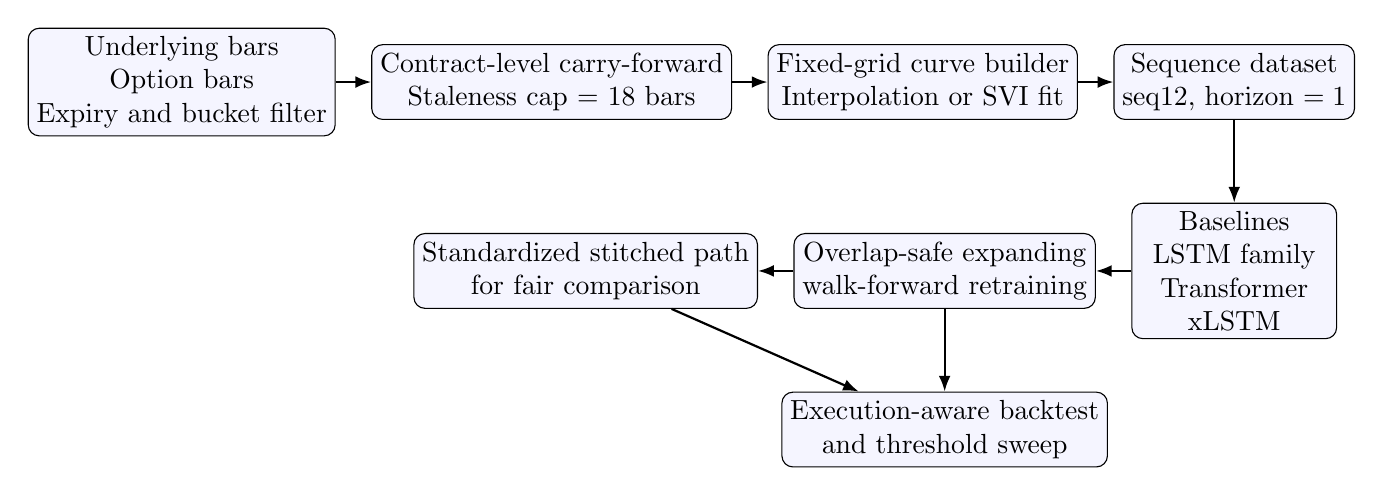
\begin{tikzpicture}[
    node distance=1.05cm and 0.45cm,
    box/.style={draw, rounded corners, align=center, minimum height=0.95cm, minimum width=2.6cm, fill=blue!4, inner sep=3pt},
    arrow/.style={-{Latex[length=2.0mm]}, thick}
]
\node[box] (raw) {Underlying bars\\Option bars\\Expiry and bucket filter};
\node[box, right=of raw] (carry) {Contract-level carry-forward\\Staleness cap = 18 bars};
\node[box, right=of carry] (curve) {Fixed-grid curve builder\\Interpolation or SVI fit};
\node[box, right=of curve] (dataset) {Sequence dataset\\seq12, horizon \(=1\)};
\node[box, below=of dataset] (models) {Baselines\\LSTM family\\Transformer\\xLSTM};
\node[box, left=of models] (wf) {Overlap-safe expanding\\walk-forward retraining};
\node[box, left=of wf] (std) {Standardized stitched path\\for fair comparison};
\node[box, below=of wf] (bt) {Execution-aware backtest\\and threshold sweep};
\draw[arrow] (raw) -- (carry);
\draw[arrow] (carry) -- (curve);
\draw[arrow] (curve) -- (dataset);
\draw[arrow] (dataset) -- (models);
\draw[arrow] (models) -- (wf);
\draw[arrow] (wf) -- (std);
\draw[arrow] (wf) -- (bt);
\draw[arrow] (std) -- (bt);
\end{tikzpicture}%
}
\caption{Methodology pipeline for the final benchmark. The study starts from intraday market data, reconstructs a denser fixed-grid IV panel, trains each model under expanding-window retraining, and evaluates both forecasting accuracy and execution-aware trading performance on one standardized out-of-sample path.}
\label{fig:pipeline}
\end{figure}

\section{Data and curve construction}
The main data-engineering challenge is not missing timestamps but cross-sectional sparsity. At many 5-minute timestamps, too few option contracts trade across moneyness to identify a stable smile slice directly. This matters because the thesis forecasts a fixed seven-node curve rather than a single scalar. If the underlying cross-section is too thin, curve quality becomes the bottleneck before modeling even begins.

The final benchmark addresses this with contract-level carry-forward. If a contract does not trade in a given 5-minute bar, its last observed option value is carried forward on the trading calendar up to a maximum staleness of 18 bars, or 90 minutes. The fill occurs at the contract level first, after which moneyness is recomputed and the fixed-grid curve is reconstructed. This is more defensible than carrying forward already-fitted grid nodes, because it preserves the link between current spot, current maturity bucket, and the contracts used to construct the smile.

The main benchmark uses this carry-forward layer together with interpolation-based curve construction. A supporting sensitivity study then replaces the interpolation layer with SVI fitting where possible. The SVI benchmark is useful because it tests whether structurally cleaner smile fitting improves the downstream ranking. As shown later, it improves the fit layer without overturning the forecasting hierarchy.

\section{Model classes}
The benchmark is intentionally broad because weak comparator sets make neural claims difficult to interpret.

\textbf{Classical and tabular baselines.} The final library includes persistence, AR(1) per grid point, factor AR/VAR, a GARCH-style ATM-shift model, ElasticNet, MLP, ExtraTrees, histogram gradient boosting, HAR factor forecasting, and a smile-coefficient baseline. These models represent local persistence, long memory, sparse linear regularization, nonlinear tabular interactions, and curve-structure preservation. They are not included as strawmen; they are included because the literature shows that such models remain strong in volatility forecasting \citep{engle1982,bollerslev1986,corsi2009,chen2024bspline}.

\textbf{Conventional LSTM.} The LSTM family provides the baseline recurrent architecture. It is a reasonable candidate because IV curves evolve through short bursts, persistence, and local path dependence. However, the dissertation does not assume that recurrence is automatically beneficial; that is part of the empirical question.

\textbf{Attention-pooled LSTM.} The attention-pooled LSTM is included as an intermediate recurrent control between plain last-hidden-state LSTM and xLSTM. It keeps the same recurrent backbone as the conventional LSTM, but replaces single-state pooling with a learned weighted summary over the sequence outputs. This tests whether part of the gap to xLSTM is explained by how temporal evidence is aggregated rather than by the memory dynamics alone.

\textbf{Transformer encoder control.} A compact transformer encoder \citep{vaswani2017} is added as a non-recurrent sequence-model control. It is important for interpretation because it separates two questions that would otherwise be conflated: whether the final result is driven by richer sequence modeling in general, or by xLSTM's particular recurrent state dynamics. In the final benchmark the transformer proves statistically competitive, even slightly better than xLSTM on RMSE, but it remains economically weaker after threshold filtering.

\textbf{xLSTM.} The xLSTM family is the architectural extension tested in this study \citep{beck2024xlstm}. The hypothesis is that a richer recurrent memory update may help separate noisy short-lived fluctuations from the smaller set of temporally coherent dislocations that matter economically. In this environment, the implemented path uses the portable \code{mLSTM}-based configuration rather than the CUDA-only \code{sLSTM} variant.

\section{Sequence-model preliminaries}
Chapter~4 serves as preliminary context, so it is useful to state the baseline recurrent update explicitly before introducing the richer sequence controls. For an input vector \(\mathbf{x}_t\), previous hidden state \(\mathbf{h}_{t-1}\), and previous cell state \(\mathbf{c}_{t-1}\), a standard LSTM computes
\begin{align}
\mathbf{i}_t &= \sigma\!\left(W_i \mathbf{x}_t + U_i \mathbf{h}_{t-1} + \mathbf{b}_i\right), \\
\mathbf{f}_t &= \sigma\!\left(W_f \mathbf{x}_t + U_f \mathbf{h}_{t-1} + \mathbf{b}_f\right), \\
\mathbf{o}_t &= \sigma\!\left(W_o \mathbf{x}_t + U_o \mathbf{h}_{t-1} + \mathbf{b}_o\right), \\
\tilde{\mathbf{c}}_t &= \tanh\!\left(W_c \mathbf{x}_t + U_c \mathbf{h}_{t-1} + \mathbf{b}_c\right), \\
\mathbf{c}_t &= \mathbf{f}_t \odot \mathbf{c}_{t-1} + \mathbf{i}_t \odot \tilde{\mathbf{c}}_t, \\
\mathbf{h}_t &= \mathbf{o}_t \odot \tanh\!\left(\mathbf{c}_t\right).
\end{align}
Here \(\mathbf{i}_t\), \(\mathbf{f}_t\), and \(\mathbf{o}_t\) are the input, forget, and output gates respectively, and \(\odot\) denotes elementwise multiplication \citep{hochreiter1997}. The practical intuition is simple: the forget gate controls what past state is retained, the input gate controls what new information is written, and the output gate controls what part of memory is exposed to the next layer or prediction head.

\subsection{Attention-pooled LSTM}
The attention-pooled LSTM keeps the same recurrent backbone, but it replaces last-state pooling with a learned weighted summary over all sequence outputs. If \(\mathbf{h}_1,\ldots,\mathbf{h}_L\) are the hidden states produced by the LSTM, the attention-pooled representation is
\begin{align}
\alpha_t &= \frac{\exp(\mathbf{q}^\top \mathbf{h}_t)}{\sum_{s=1}^{L}\exp(\mathbf{q}^\top \mathbf{h}_s)}, \\
\bar{\mathbf{h}} &= \sum_{t=1}^{L}\alpha_t \mathbf{h}_t,
\end{align}
where \(\mathbf{q}\) is a learned scoring vector. This is a standard self-attentive pooling form adapted from sequence-attention architectures such as those of Lin et al.~\citep{lin2017selfattentive}. The point of this variant is not to introduce a fundamentally different model family, but to test whether better temporal aggregation alone can close part of the gap between plain LSTM and xLSTM.

\subsection{Transformer encoder control}
The transformer encoder control removes recurrence entirely and relies on self-attention across the lookback window \citep{vaswani2017}. With an input projection \(W_{\text{in}}\) and positional embedding \(\mathbf{p}_t\), the initial token state is
\[
\mathbf{z}^{(0)}_t = W_{\text{in}}\mathbf{x}_t + \mathbf{p}_t.
\]
Each encoder block then applies self-attention and a feed-forward update,
\begin{align}
\tilde{\mathbf{z}}^{(\ell)} &= \mathrm{MHA}\!\left(\mathbf{z}^{(\ell-1)}\right) + \mathbf{z}^{(\ell-1)}, \\
\mathbf{z}^{(\ell)} &= \mathrm{FFN}\!\left(\tilde{\mathbf{z}}^{(\ell)}\right) + \tilde{\mathbf{z}}^{(\ell)},
\end{align}
followed by normalization, following the encoder structure introduced by Vaswani et al.~\citep{vaswani2017}. In this dissertation the transformer is not the headline model; it is a high-quality non-recurrent control used to separate generic sequence-modeling gains from xLSTM-specific recurrent gains.

\subsection{xLSTM intuition}
The xLSTM family keeps the recurrent framing but replaces the standard memory update with a richer state-transition design intended to improve stability and scaling \citep{beck2024xlstm}. At a high level, it can be written as
\begin{align}
\mathbf{s}_t &= G_\theta(\mathbf{x}_t, \mathbf{s}_{t-1}, \mathbf{h}_{t-1}), \\
\mathbf{h}_t &= F_\theta(\mathbf{x}_t, \mathbf{s}_t, \mathbf{h}_{t-1}),
\end{align}
where \(\mathbf{s}_t\) denotes the internal memory state and \(F_\theta, G_\theta\) are richer transition maps than those in the standard LSTM. These equations are schematic abstractions of the richer recurrent transition proposed by Beck et al.~\citep{beck2024xlstm}; they are included here only to convey the role of the latent state update rather than to reproduce the full block definition. The reader does not need to follow every implementation detail of the underlying \code{mLSTM} block. The important point is conceptual: xLSTM is tested because its memory dynamics may preserve temporally coherent, economically meaningful dislocations better than a plain last-state LSTM, even if it does not win on average forecast loss.

\chapter{Experimental Design}

\section{Main benchmark}
The empirical design is organized around one main experiment and one supporting sensitivity check. The main experiment is the 5-minute carry-forward benchmark with one standardized out-of-sample path, the full baseline library, the recurrent-model family, the transformer control, and the xLSTM extension under the same execution rules. This is the experiment from which the headline findings are drawn.

Table~\ref{tab:design_summary} summarizes the main design.

\begin{table}[H]
\centering
\caption{Main experimental design for the dissertation's primary benchmark.}
\label{tab:design_summary}
\footnotesize
\renewcommand{\arraystretch}{1.15}
\begin{tabularx}{\textwidth}{@{}lY@{}}
\toprule
\textbf{Component} & \textbf{Specification} \\
\midrule
Underlying & SPY \\
Sampling frequency & 5-minute bars \\
Target maturity bucket & 30 \(\pm\) 7 days to expiry \\
Forecast target & Seven-node fixed moneyness IV curve \\
Moneyness grid & \(-0.15,-0.10,-0.05,0.00,0.05,0.10,0.15\) \\
Supervised dataset size & 50,019 samples (carry-forward benchmark) \\
Sequence / horizon & seq12, one-bar ahead \\
Model families & 10 baselines, 4 vanilla LSTM variants, 1 attention-pooled LSTM, 1 transformer encoder, 4 xLSTM variants \\
Validation design & 15-fold expanding walk-forward, overlap-safe frontier stitching \\
Economic layer & Execution-aware backtest with exposure caps and transaction costs \\
Reporting views & Fixed threshold benchmark and descriptive threshold sweep \\
\bottomrule
\end{tabularx}
\end{table}

This design reflects the core thesis objective. It is not simply a forecasting contest. It is a benchmark built to distinguish models that minimize average error from models that produce actionable, high-conviction mispricing signals.


\section{Validation and evaluation}
The final carry benchmark uses the 5-minute carry-forward dataset with 50,019 supervised samples, sequence length 12, and one-bar-ahead targets. The walk-forward split uses:
\begin{itemize}[leftmargin=1.2cm]
    \item initial train size: 17,630;
    \item validation size: 3,526;
    \item test size: 3,526;
    \item step size: 1,763;
    \item overlap-safe frontier stitching.
\end{itemize}
This produces 15 expanding-window folds without duplicated timestamps in the stitched out-of-sample path.

Two economic views are reported. The first is a fixed-threshold benchmark at \(\tau=0.0015\), which answers the question: under one common decision rule, which model is strongest? The second is a descriptive threshold sweep over
\[
\tau \in \{0.0015,0.0020,0.0025,0.0030,0.0040,0.0050,0.0075,0.0100\},
\]
which answers a different question: which models produce the most useful high-confidence signals once weak actions are filtered out? This second view matters because an options desk often cares more about the quality of a sparse actionable subset than about small average errors near zero.

\section{Evaluation metrics}
The statistical and economic metrics play different roles, so the benchmark reports both. For the realized curve \(\mathbf{c}_t\) and forecast \(\hat{\mathbf{c}}_t\), root mean squared error is
\[
\mathrm{RMSE}=\sqrt{\frac{1}{N}\sum_{t=1}^{N}\lVert \hat{\mathbf{c}}_t-\mathbf{c}_t\rVert_2^2},
\]
mean absolute error is
\[
\mathrm{MAE}=\frac{1}{N}\sum_{t=1}^{N}\lVert \hat{\mathbf{c}}_t-\mathbf{c}_t\rVert_1,
\]
and the coefficient of determination is
\[
R^2 = 1 - \frac{\sum_{t=1}^{N}\lVert \hat{\mathbf{c}}_t-\mathbf{c}_t\rVert_2^2}{\sum_{t=1}^{N}\lVert \mathbf{c}_t-\bar{\mathbf{c}}\rVert_2^2},
\]
where \(\bar{\mathbf{c}}\) is the sample mean curve over the evaluation path. RMSE and MAE follow the standard forecast-accuracy definitions summarized by Hyndman and Koehler~\citep{hyndman2006}, while \(R^2\) is reported in the usual proportion-of-variance-explained form for multivariate regression output.

The economic layer reports tuned net PnL, tuned Sharpe, maximum drawdown, directional edge accuracy, and signal-realized correlation. Net PnL is defined operationally for this benchmark as post-cost cumulative trading profit,
\[
\mathrm{PnL}_{\mathrm{net}}(\tau)=\sum_{t\in\mathcal{T}_\tau}\big(\pi_t-\kappa_t\big),
\]
where \(\pi_t\) denotes gross trade PnL and \(\kappa_t\) denotes the transaction-cost deduction implied by the execution model. Sharpe is reported as
\[
\mathrm{Sharpe}=\frac{\mathbb{E}[r_t]}{\mathrm{sd}(r_t)},
\]
where \(r_t\) denotes the strategy return series on the standardized path, following the standard excess-return normalization in Sharpe~\citep{sharpe1994}. Maximum drawdown is the worst peak-to-trough loss on cumulative net PnL,
\[
\mathrm{MDD}=\min_t\left(P_t-\max_{s\le t}P_s\right),
\]
where \(P_t\) denotes cumulative net PnL. This is the standard peak-to-trough risk summary used in performance reporting; in this dissertation it is implemented directly from the cumulative strategy path rather than imported as a separate theoretical object. To define directional edge accuracy, let the realized vega-weighted edge score be
\[
\tilde{s}_t=\sum_{j=1}^{7} w_j \big(c_{t+1,j}-c_{t,j}\big),
\]
and let the traded set under threshold \(\tau\) be
\[
\mathcal{T}_\tau=\{t:\lvert s_t\rvert>\tau\}.
\]
Directional edge accuracy is then
\[
\mathrm{DEA}(\tau)=\frac{1}{|\mathcal{T}_\tau|}\sum_{t\in\mathcal{T}_\tau}\mathbf{1}\!\left[\operatorname{sign}(s_t)=\operatorname{sign}(\tilde{s}_t)\right].
\]
It therefore measures whether the sign of the predicted vega-weighted edge agrees with the sign of the realized edge on the traded subset generated by the selected threshold-swept strategy. This is a benchmark-specific metric introduced in the dissertation because standard forecast losses do not directly capture whether the monetized edge is directionally correct on the sparse traded subset. The benchmark also logs the signal-realized correlation, reported as the standard Pearson correlation between the scalar forecast signal \(s_t\) and the realized edge score \(\tilde{s}_t\) across the full path. It is useful diagnostically as a ranking-quality statistic, but the main results table emphasizes the more interpretable drawdown and directional-edge metrics. In this dissertation, the key interpretation is simple: RMSE, MAE, and \(R^2\) ask how well the full curve is forecast on average, while the economic metrics ask whether the forecast errors translate into selective, monetizable trades.

\section{Why the execution layer is a reasonable abstraction}
The execution layer is stylized, but it is not arbitrary. The scalar score \(s_t\) is a vega-weighted aggregation because a fixed-maturity smile forecast has to be collapsed into a direction that is interpretable in risk terms. A vega-style weighting is a reasonable first-order approximation for turning a multi-node curve forecast into a tradeable scalar without pretending that the benchmark is a full contract-level options book. The one-bar holding rule is intentionally short. It isolates immediate mispricing correction instead of allowing a model to benefit from slower multi-bar drift, regime drift, or inventory-style carry that would blur the link between next-bar IV adjustment and realized trading outcome.

Thresholding is equally important. On this benchmark, near-zero forecast scores are often economically indistinguishable from noise once transaction costs are applied. The threshold sweep is therefore not cosmetic tuning; it is part of the identification problem. The contrast between the conventional LSTM and the xLSTM family makes this clear. Weak recurrent forecasts can produce thousands of low-quality trades and strongly negative post-cost PnL, while a more selective model can remain economically positive even without dominating RMSE. Position limits and exposure caps serve the same purpose. They prevent the benchmark from manufacturing performance through turnover and leverage rather than through better signal ranking.

The friction model is intentionally conservative rather than highly customized. The base configuration uses a 17-bps round-trip cost and is stressed further through wider-spread and latency-proxy scenarios taken from the completed appendix pack. Table~\ref{tab:execution_sensitivity_main} shows that the economic ordering is not especially fragile to these cost-side stresses: net PnL compresses for the whole frontier, but the winner does not change.

\begin{table}[H]
\centering
\caption{Execution-sensitivity check for the main frontier under the completed cost-side stress scenarios. Net PnL is reported for each model under its selected threshold.}
\label{tab:execution_sensitivity_main}
\footnotesize
\renewcommand{\arraystretch}{1.15}
\begin{tabular*}{\textwidth}{@{\extracolsep{\fill}} l r r r r l @{}}
\toprule
\textbf{Scenario} & \textbf{xLSTM} & \textbf{ElasticNet} & \textbf{HAR} & \textbf{MLP} & \textbf{Winner} \\
\midrule
Base (17 bps) & 0.1213 & 0.1109 & 0.1146 & 0.1156 & xLSTM \\
Wider spread (23 bps) & 0.1081 & 0.0963 & 0.1009 & 0.0916 & xLSTM \\
Latency proxy (25 bps) & 0.1037 & 0.0915 & 0.0964 & 0.0836 & xLSTM \\
Combined stress (31 bps) & 0.0905 & 0.0769 & 0.0827 & 0.0596 & xLSTM \\
\bottomrule
\end{tabular*}
\end{table}

This robustness table does not prove that the backtest is a deployable execution simulator. It does show that the conclusion is not being carried by one unusually cheap friction assumption. A longer holding horizon or a full contract-level simulator would answer a different question and would be appropriate future work, but they are not needed to justify the current benchmark as a disciplined short-horizon abstraction.

\section{Robustness design}
Several layers of rigor are included, but each one answers a different question. The completed evidence includes standardized walk-forward comparison, fixed-threshold and threshold-swept backtests, a winner-versus-all-competitors appendix pack for the final xLSTM, pairwise Diebold--Mariano predictive-accuracy tests \citep{diebold1995}, and a block-bootstrap significance analysis for tuned net PnL and Sharpe on the final economic frontier. The appendix pack reports matched moneyness-region, regime-split, and execution-sensitivity comparisons against the full comparison library on the standardized carry-forward window, including the transformer and attention-pooled LSTM controls in addition to the classical baselines. The carry-plus-SVI experiment serves as a targeted data-layer sensitivity check. Together, these layers support a disciplined claim: the final xLSTM is the realized economic winner on the main carry benchmark, but it does not become the dominant statistical forecaster and it does not separate cleanly from the strongest challenger cluster on every inferential view.

\section{Implementation architecture}
The system is implemented as a modular pipeline with four layers:
\begin{enumerate}[leftmargin=1.2cm]
    \item data-provider and preprocessing modules for underlying bars, option bars, carry-forward, and curve fitting;
    \item dataset builders for fixed-grid supervised sequences;
    \item model modules for baselines, conventional LSTM, attention-pooled LSTM, transformer, and xLSTM;
    \item evaluation modules for walk-forward training, standardized stitching, statistical testing, and backtesting.
\end{enumerate}

The project repository associated with this dissertation is available at \url{https://github.com/shamesjen/fyp}. It contains the data-processing scripts, model definitions, experiment configurations, and figure-generation code used to produce the reported results.

This material is kept in the experimental-design chapter rather than in the early conceptual framing because it is part of reproducibility, not problem definition. The implementation separation matters empirically: it allows the dissertation to change the data layer, such as switching from interpolation to SVI, without rewriting the downstream model-training and evaluation stack.

\section{Carry-plus-SVI sensitivity}
One focused sensitivity study replaces the carry-only interpolation layer with carry plus SVI smoothing. The purpose is to test whether a more structured smile-construction layer improves the downstream model ranking. The SVI study is interpreted as evidence about the \emph{data layer} rather than as the final architecture-selection benchmark, because the main carry-forward experiment remains the central comparison.

\chapter{Results and Analysis}

\section{Statistical and economic winners differ}
Table~\ref{tab:main_results} presents the core result of the dissertation. The fixed-threshold benchmark remains useful as a common-rule check, but the main decision-relevant comparison is the threshold-swept benchmark, where each model is evaluated on the same standardized path at its own descriptive best threshold. The central question is not whether every small signal should be traded, but whether the strongest signals can be converted into stable post-cost edge.

\begin{table}[H]
\centering
\caption{Selected main final carry-forward results across the strongest baselines and the most relevant neural controls on the standardized seq12 one-bar-ahead path. All non-RMSE columns are computed from each model's selected threshold-swept strategy on the same standardized prediction path. Directional edge accuracy is therefore a trade-conditional quantity under the selected threshold, not an all-bar percentage. Best values are shown in bold and second-best values are underlined.}
\label{tab:main_results}
\scriptsize
\setlength{\tabcolsep}{4pt}
\renewcommand{\arraystretch}{1.15}
\begin{tabular*}{\textwidth}{@{\extracolsep{\fill}} l r r r r r @{}}
\toprule
\textbf{Model} & \textbf{Tuned net PnL} & \textbf{Tuned Sharpe} & \textbf{RMSE} & \textbf{Max DD} & \textbf{Dir. edge acc.} \\
\midrule
xLSTM b2/e256 (proposed method) & \textbf{0.121296} & \textbf{3.876124} & 0.013914 & \textbf{-0.004344} & \textbf{0.693182} \\
Transformer 2/128/4 & 0.103707 & 3.172473 & 0.013660 & -0.016524 & 0.625000 \\
Attn.\ LSTM 2x128 & 0.034551 & 1.090924 & 0.034425 & -0.077584 & 0.594891 \\
LSTM 2x128 & -0.386723 & -10.341794 & 0.033279 & -0.492919 & 0.524696 \\
ElasticNet & 0.110865 & 3.494970 & \textbf{0.010886} & -0.007632 & 0.639175 \\
MLP & \uline{0.115634} & 3.479333 & \uline{0.012646} & -0.014310 & 0.631250 \\
HAR factor & \uline{0.114551} & \uline{3.607436} & 0.013573 & \uline{-0.007299} & 0.648352 \\
Smile coefficient & 0.109536 & 3.510701 & 0.020815 & -0.007382 & \uline{0.679012} \\
HistGB & 0.043282 & 1.516405 & 0.013726 & -0.043538 & 0.603448 \\
\bottomrule
\end{tabular*}
\vspace{0.4em}

{\footnotesize\emph{Interpretation.} ElasticNet is the statistical leader and remains near the economic frontier. xLSTM becomes the strongest tuned economic model after threshold filtering and also leads the displayed frontier on Sharpe, drawdown control, and directional edge accuracy. The transformer encoder is statistically strong and economically positive, but it still remains below the xLSTM on the tuned economic view. The attention-pooled LSTM improves materially over the vanilla LSTM, but it still does not approach the xLSTM frontier on any of the key economic metrics.}
\end{table}

\insertassetfigure{Final carry-forward benchmark trade-off between statistical accuracy and tuned economic value across the strongest baselines, the transformer encoder control, and the winning xLSTM. The vanilla LSTM and attention-pooled LSTM controls are omitted from the plot because they are large outliers on both axes and would compress the main frontier cluster. ElasticNet remains the statistical leader on RMSE, while xLSTM becomes the strongest model by tuned net PnL after threshold filtering.}{fig:tradeoff}{fig_carry_retuned_tradeoff.png}

The benchmark does not support a blanket statement that recurrent models dominate classical alternatives. ElasticNet is the best average forecaster on the standardized test path. xLSTM becomes the strongest economic model only after the signal is filtered for high-confidence actions. The model that best minimizes average error is not necessarily the model that produces the best monetizable edge under cost.

The trade-side directional metric in Table~\ref{tab:main_results} should be read in that same thresholded sense. It is not computed over all evaluation bars. It is computed on the executed trades generated by each model's selected threshold-swept strategy. This is why the plain LSTM can still look directionally reasonable on a subset of trades and yet remain economically poor once drawdown and post-cost PnL are taken seriously.

The rest of the frontier is also informative. MLP, HAR factor forecasting, and the smile-coefficient baseline remain close to the tuned economic frontier, which reinforces the point that this is a hard benchmark and that the comparator library is not weak. In the completed winner-versus-all-competitors test, the xLSTM lead is 0.0104 net PnL over ElasticNet, 0.0067 over HAR, 0.0057 over MLP, 0.0118 over the smile-coefficient baseline, and 0.0176 over the transformer control on the same standardized path after each model is evaluated at its own best threshold. Those margins support xLSTM as the realized winner, but not as a runaway winner. The single transformer encoder control is also informative. It reaches RMSE 0.01366, which is slightly better than the final xLSTM's 0.01391, but its tuned net PnL remains lower at 0.1037 and its max drawdown is materially worse at \(-0.0165\). The attention-pooled LSTM shows that some of the gap between plain LSTM and xLSTM can be closed by replacing last-hidden-state pooling with learned sequence pooling, but the improvement is still modest. The best attention-pooled LSTM reaches tuned net PnL 0.0346 and Sharpe 1.09, which is directionally positive yet still far from the xLSTM and the top challenger cluster.

\section{xLSTM after thresholding}
The best xLSTM does not win by trading more often. It wins by becoming more selective. On the final carry-forward benchmark, xLSTM b2/e256 is strongest at threshold \(\tau=0.0050\), not at the fixed benchmark threshold of 0.0015. Under that stricter setting it generates only 88 trades across 28,208 evaluation periods and reaches Sharpe 3.876. The attention-pooled LSTM requires the stricter threshold \(\tau=0.0100\) and still reaches only 274 trades, Sharpe 1.09, and max drawdown \(-0.0776\). The best plain last-hidden-state LSTM remains negative even at the same high threshold.

The economic advantage is driven by selectivity and payoff asymmetry. At the selected threshold, the xLSTM's average positive trade contribution is approximately 0.00353, while its average negative trade contribution is only about \(-0.00059\). This is why the model can remain economically strong even without dominating every forecasting metric: the high-confidence subset is small, but the favorable trades are much larger in magnitude than the unfavorable ones. Directional edge accuracy captures this more cleanly because it focuses on whether the sign of the monetized edge is correct on the traded subset.

\insertassetfigure{Thresholded xLSTM equity curve on the final carry-forward benchmark. The plot corresponds to xLSTM b2/e256 at its best descriptive threshold \(\tau=0.0050\). The important feature is selectivity and smoothness rather than the absolute scale of cumulative PnL.}{fig:xlstm_equity}{fig_xlstm_thresholded_equity_curve.png}

Figure~\ref{fig:xlstm_equity} illustrates the practical implication. The xLSTM does not dominate the entire score distribution. Instead, it appears to rank the extreme tail of opportunities better than the conventional LSTM, and well enough to overtake the top baselines on tuned net PnL. This matters because the economic layer is vega-weighted and cost-sensitive. Once trades are thresholded, the value of a model depends less on small errors near zero and more on whether its largest predicted dislocations correspond to genuinely tradable events.

This is also the strongest conceptual reason for including xLSTM in the dissertation. A richer recurrent memory block is justified here not because it guarantees better average forecasting, but because it may better preserve regime persistence, local state shifts, and transient but economically relevant intraday structure. The evidence in this dissertation is consistent with that interpretation. It is not a mechanistic proof of what the memory block learns, but it is a coherent empirical reason why economic leadership can differ from statistical leadership.

\section{Economic significance and deployment value}
The xLSTM result matters most as a statement about ranking quality, not as evidence of a large standalone trading edge. The tuned net-PnL advantage over ElasticNet on the standardized path is 0.0104, over HAR 0.0067, over MLP 0.0057, and over the transformer control 0.0176. Those margins are economically positive, but they are small relative to the overall spread of the benchmark and they remain narrow under bootstrap resampling. The practical interpretation is that xLSTM improves the selection of the highest-conviction events at the margin; it does not render the strongest baselines obsolete.

The absolute PnL units in this benchmark are normalized by the execution layer and should not be read as deployable dollar profits. What they do support is an ordering among models under the same assumptions. From a desk perspective, that ordering matters only if the improvement is large enough to justify added complexity, monitoring, and model-risk cost. Table~\ref{tab:practical_ranking} summarizes the trade-off. xLSTM is strongest on the tuned economic metrics, but ElasticNet remains the simplest and statistically strongest default, while HAR and MLP remain close economic challengers.

\begin{table}[H]
\centering
\caption{Practical reading of the main frontier. Rank columns are computed on the full final carry benchmark, not only within the displayed subset.}
\label{tab:practical_ranking}
\footnotesize
\renewcommand{\arraystretch}{1.15}
\setlength{\tabcolsep}{3pt}
\begin{tabularx}{\textwidth}{@{}>{\RaggedRight\arraybackslash}p{0.19\textwidth}>{\centering\arraybackslash}p{0.09\textwidth}>{\centering\arraybackslash}p{0.08\textwidth}>{\centering\arraybackslash}p{0.10\textwidth}>{\RaggedRight\arraybackslash}p{0.18\textwidth}Y@{}}
\toprule
\textbf{Model} & \textbf{\shortstack[c]{RMSE\\rank}} & \textbf{\shortstack[c]{PnL\\rank}} & \textbf{\shortstack[c]{Sharpe\\rank}} & \textbf{Complexity} & \textbf{\shortstack[l]{Practical\\takeaway}} \\
\midrule
xLSTM b2/e256 & 10 & 1 & 1 & High, recurrent & Best economic model on the completed benchmark; useful if the desk values sparse high-conviction signals enough to justify a more complex recurrent model. \\
ElasticNet & 1 & 4 & 4 & Low, sparse linear & Best statistical benchmark and still very close economically; strongest low-complexity default. \\
HAR factor & 6 & 3 & 2 & Low, linear multi-horizon & Strong risk-adjusted challenger with simple dynamics and easy interpretation. \\
MLP & 5 & 2 & 5 & Medium, tabular neural & Economically close to xLSTM, but with weaker drawdown control and less interpretability than the linear challengers. \\
Transformer 2/128/4 & 7 & 6 & 8 & Medium-high, attention encoder & Strong non-recurrent control; good statistical fit, but economically weaker than xLSTM on the same path. \\
\bottomrule
\end{tabularx}
\end{table}

The bootstrap evidence keeps this interpretation disciplined. xLSTM's own tuned net-PnL interval stays positive, but the pairwise intervals against ElasticNet, HAR, MLP, the smile-coefficient baseline, and the transformer all cross zero. A practitioner should read that as evidence of a competitive economic lead rather than a decisive deployable edge. The practical value of the model is improved identification of high-confidence dislocations under the benchmark's execution rules, not proof that the model would dominate a fully specified production desk without further work.

\section{Vanilla LSTM failure mode}
The plain LSTM problem is not merely undertraining. The best vanilla carry-forward configuration, LSTM \(2\times128\), reaches RMSE 0.0333, tuned net PnL \(-0.3867\), Sharpe \(-10.34\), and max drawdown \(-0.4929\). Its directional edge accuracy remains only 0.5247, well below the xLSTM winner and only modestly above random sign agreement.

That pattern is informative. The result is not that recurrence is useless. It is that the form of recurrence matters. The conventional LSTM appears to convert moderate score fluctuations into too many weak trades with poor post-cost expectancy. Even when some trade directions are locally correct, the resulting strategy still suffers large drawdowns and strongly negative net PnL. In contrast, the best xLSTM configuration behaves more like a sparse scoring model: fewer trades, stronger average conviction, and better conversion of forecast variation into monetizable edge.

\section{Attention-pooled LSTM as an intermediate control}
The attention-pooled LSTM creates the intermediary that the plain LSTM family was missing. Relative to the vanilla LSTM, it improves the tuned net PnL from \(-0.3867\) to \(0.0346\), improves Sharpe from \(-10.34\) to \(1.09\), and reduces maximum drawdown from \(-0.4929\) to \(-0.0776\). This is a substantial improvement and it shows that the pooling choice matters.

The result also clarifies what attention pooling does \emph{not} solve. The model still remains far from the frontier established by xLSTM and the strongest baselines. Its RMSE remains poor at 0.0344, its directional edge accuracy stays below 0.60, and it requires a relatively strict threshold \(\tau=0.0100\) to become positive at all. The natural interpretation is that learned pooling helps the model summarize the short sequence more sensibly than a single last hidden state, but it does not fully resolve the underlying problem of producing calibrated high-conviction intraday signals.

\section{Transformer control and statistical-economic divergence}
The transformer encoder control is the strongest non-recurrent neural comparator in the study. It reaches RMSE 0.01366, slightly better than xLSTM's 0.01391, while remaining economically positive after thresholding with tuned net PnL 0.1037 and Sharpe 3.17. On pure forecast accuracy this is a strong result.

At the same time, the transformer does not overtake xLSTM on the economic view. Its tuned net PnL remains below the xLSTM winner, its maximum drawdown is worse at \(-0.0165\), and its directional edge accuracy stays lower at 0.6250 versus xLSTM's 0.6932. This is an important control result because it shows that the final conclusion is not simply ``more expressive sequence models do better.'' The transformer can improve average full-curve fit, but the xLSTM still appears better at isolating the subset of large, tradable dislocations that survive thresholding and cost.

\section{SVI sensitivity}
The carry-plus-SVI sensitivity is useful because it separates structural smile fitting from downstream predictive value. Contract-level carry-forward makes SVI feasible on most slices, which means the SVI experiment is not failing merely because the smile cannot be calibrated.

\insertassetfigure{Fit-method mix in the SVI carry panel. Contract-level carry-forward makes direct SVI fitting feasible on 92.8\% of rows, so the sensitivity genuinely tests a structure-aware curve layer rather than a mostly failed calibration routine.}{fig:svi_fit_mix}{fig_svi_carry_fit_mix.png}

Figure~\ref{fig:svi_fit_mix} shows that 46,427 of 50,031 rows in the SVI panel are direct SVI fits, with only 2,760 interpolation fallbacks and 844 flat-fill cases. The data layer is therefore materially improved relative to the earlier sparse panel. Yet the downstream ranking still does not improve. In the carry benchmark, ElasticNet achieves RMSE 0.010886 and xLSTM b2/e256 achieves RMSE 0.015034. In the SVI benchmark, those values worsen to 0.015476 and 0.019468 respectively. Economically, ElasticNet remains the leader in the completed SVI family benchmark, and xLSTM remains the best neural model but falls further behind.

The right interpretation is not that SVI is mathematically wrong. It is that structurally cleaner curve fitting does not automatically create a better prediction target for this task. On this dataset, the bottleneck remains the extraction of a stable, monetizable short-horizon signal, not only the smoothness of the fitted smile.

\section{Diebold--Mariano predictive-accuracy tests}
Pairwise Diebold--Mariano tests \citep{diebold1995} on the carry-forward appendix pack show that xLSTM b2/e256 does \emph{not} become the dominant statistical forecaster once it is compared against the full challenger set on the same standardized path. ElasticNet still defeats xLSTM decisively on overall and ATM forecast loss, with DM statistic \(31.75\) overall and \(10.73\) at ATM, both with \(p=0.0\). xLSTM also loses overall to AR(1), persistence, GARCH, MLP, and HAR. Conversely, it beats ExtraTrees, smile-coefficient forecasting, and factor AR/VAR on overall loss, and it outperforms MLP, ExtraTrees, histogram gradient boosting, factor AR/VAR, and the smile-coefficient baseline on the ATM node. In the carry-plus-SVI family comparison, the same basic pattern remains: ElasticNet stays ahead statistically, with overall DM statistic \(-24.18\) in its favor against xLSTM and \(p=0.0\).

This distinction is the substantive finding of the study. Once transaction costs, thresholding, and exposure limits are introduced, not all forecast errors matter equally. Small errors around zero are often economically irrelevant. A model can lose on average squared error yet still win economically if it places the most extreme predicted dislocations in the right places. The benchmark is designed precisely to reveal that possibility.

\section{Region and regime interpretation}
The xLSTM advantage is not broad-based statistical domination across regions or regimes. It remains weaker than ElasticNet in both high-ATM-IV and low-ATM-IV regimes on forecast RMSE. Against some nonlinear baselines, however, the pattern is more mixed: xLSTM improves on histogram gradient boosting in the low-ATM-IV regime and on several baselines around ATM, while remaining weaker on other regions such as the put wing. The non-recurrent controls sharpen this interpretation further. Against the transformer control, overall DM favors the transformer on full-curve forecast loss with statistic 5.98 and \(p \approx 2.3\times10^{-9}\), while ATM DM favors xLSTM with statistic \(-5.59\) and \(p \approx 2.3\times10^{-8}\). Against the attention-pooled LSTM, xLSTM wins decisively on both overall and ATM loss with effectively zero \(p\)-values. That is exactly the profile one would expect from a model whose strength lies in ranking a useful subset of dislocations rather than minimizing average error everywhere.

\section{Bootstrap significance of the economic frontier}
A block-bootstrap significance check strengthens the economic interpretation while also making the remaining uncertainty explicit. Using 1,000 circular block-bootstrap replications with one-trading-day blocks, xLSTM b2/e256 retains a 95\% confidence interval of \([0.0703, 0.1710]\) for tuned net PnL and \([2.8983, 4.6860]\) for Sharpe, with bootstrap probability 1.0 of positive net PnL and positive Sharpe. The transformer control is also robustly positive on its own path, with tuned net-PnL confidence interval \([0.0543, 0.1585]\) and Sharpe confidence interval \([1.8720, 4.3302]\). This is strong evidence that the xLSTM signal is genuinely positive on the observed path rather than an artifact of a single favorable run, but it also shows that the strongest alternatives remain economically credible.

\insertassetfigure{Block-bootstrap confidence intervals for tuned net PnL on the final carry-forward frontier. xLSTM b2/e256 is robustly positive, but the transformer control and the top baseline cluster remain close and also retain positive intervals.}{fig:bootstrap_pnl}{fig_bootstrap_net_pnl_ci.png}

The bootstrap also clarifies the competitive structure of the frontier. The xLSTM lead over histogram gradient boosting and ExtraTrees remains clearly positive under resampling, but the lead over the strongest challenger cluster is much tighter. The 95\% net-PnL delta intervals versus the transformer control \([{-}0.0075, 0.0467]\), ElasticNet \([{-}0.0087, 0.0327]\), HAR \([{-}0.0119, 0.0272]\), MLP \([{-}0.0196, 0.0365]\), and the smile-coefficient baseline \([{-}0.0074, 0.0331]\) all cross zero, even though the realized xLSTM point estimate stays ahead in each case. In probability terms, the bootstrap assigns xLSTM a 0.903 chance of beating the transformer on tuned net PnL and a 0.942 chance of beating it on tuned Sharpe; those probabilities support the economic ranking without implying clean separation.

\insertassetfigure{Block-bootstrap confidence intervals for the xLSTM net-PnL lead over the strongest challengers. The vertical axis lists challenger models, so positive values indicate that xLSTM b2/e256 remains ahead on the observed path. The figure shows that the realized economic win is positive, but its margin over the transformer control and the top baseline cluster is narrow rather than statistically cleanly separated.}{fig:bootstrap_delta}{fig_bootstrap_winner_delta_ci.png}

xLSTM is the realized economic winner on the main carry benchmark, and its own positive performance is well supported by the bootstrap. At the same time, the economic frontier with the transformer control, ElasticNet, HAR, MLP, and the smile-coefficient baseline remains tight. This keeps the dissertation's claim disciplined: xLSTM is the strongest tuned economic model in the completed benchmark, but the result is best understood as leadership within a competitive frontier rather than decisive universal dominance.

\chapter{Discussion, Limitations, and Future Work}

\section{Implications}
The main implication of the dissertation is that option desks and ML researchers should not treat point forecasting and tradable signal extraction as identical tasks. A desk cares about confidence, execution feasibility, and stable monetizable edge, not only average loss. The benchmark here makes that explicit. ElasticNet is the best statistical model on the main test path, yet xLSTM becomes the best economic model after the decision layer is filtered. That is not a contradiction. It is exactly what one should expect when the objective is to trade only the strongest dislocations.

This matters operationally. A desk may rationally prefer a model that produces fewer, more stable, higher-conviction signals over one that is incrementally better on average RMSE but noisier near the trading threshold. In a cost-sensitive environment, lower-variance signal extraction can be more useful than globally lower error. The study therefore argues for a broader definition of model quality in intraday options work.

\section{Limitations}
The study also has clear limits.
\begin{enumerate}[leftmargin=1.3cm]
    \item Intraday listed-option data remain sparse across strikes and maturities, even after contract-level carry-forward. The benchmark also excludes OTC option activity and quote-book information, so the observed smile is an incomplete view of the full market.
    \item The economic layer is execution-aware but still stylized. It is not a contract-level order-book simulator and it does not hold options to expiry.
    \item The SVI evidence is best interpreted as a curve-construction sensitivity rather than as a final matched neural retune. It is informative about the data layer, but it does not supersede the main carry benchmark.
\end{enumerate}

\section{Future work}
The most natural extensions follow directly from these limits. The first is a richer decomposition of where the economic advantage appears, especially across moneyness regions, market regimes, and time of day. The second is a matched placebo-and-ablation suite on the final winner so that the role of carry-forward, thresholding, and execution frictions can be isolated under the exact same benchmark. The third is a more structure-aware target, such as coefficient or parameter forecasting, so that structural smile information is not used only in preprocessing. The fourth is broader validation across additional liquid underlyings and maturity buckets.

\section*{Concluding remarks}
The study examined intraday implied-volatility curve forecasting as a trading-relevant forecasting problem. Strong baselines, especially ElasticNet, remain the statistical benchmark. xLSTM b2/e256 becomes the strongest economic model on the main carry benchmark after high-confidence filtering, while the conventional LSTM family remains materially weaker and the transformer control shows that slightly better statistical accuracy need not imply the best monetized strategy. The completed appendix and bootstrap evidence sharpen that picture: the xLSTM signal itself is robustly positive, but its advantage over the strongest challenger cluster is narrow rather than overwhelming. The main contribution is a unified leakage-aware and execution-aware benchmark that makes this divergence between statistical accuracy and economic usefulness observable on a common path.

\cleardoublepage
\addcontentsline{toc}{chapter}{References}
\begin{thebibliography}{99}

\bibitem{black1973}
Black, F. and Scholes, M. (1973).
\newblock The pricing of options and corporate liabilities.
\newblock \emph{Journal of Political Economy}, 81(3), 637--654.

\bibitem{dumas1998}
Dumas, B., Fleming, J., and Whaley, R.~E. (1998).
\newblock Implied volatility functions: Empirical tests.
\newblock \emph{The Journal of Finance}, 53(6), 2059--2106.

\bibitem{gu2020}
Gu, S., Kelly, B., and Xiu, D. (2020).
\newblock Empirical asset pricing via machine learning.
\newblock \emph{The Review of Financial Studies}, 33(5), 2223--2273.

\bibitem{heaton2017}
Heaton, J.~B., Polson, N.~G., and Witte, J.~H. (2017).
\newblock Deep learning in finance.
\newblock arXiv preprint arXiv:1602.06561.

\bibitem{arratia2025}
Arratia, A., El Daou, M., Kagerhuber, J., and Smolyarova, Y. (2025).
\newblock Examining challenges in implied volatility forecasting: A critical review of data leakage and feature engineering combined with high-complexity models.
\newblock \emph{Computational Economics}.

\bibitem{beck2024xlstm}
Beck, M., P\"oppel, K., Spanring, M., Auer, A., Prudnikova, O., Kopp, M., Klambauer, G., Brandstetter, J., and Hochreiter, S. (2024).
\newblock xLSTM: Extended Long Short-Term Memory.
\newblock arXiv preprint arXiv:2405.04517.

\bibitem{bernales2014}
Bernales, A. and Guidolin, M. (2014).
\newblock Can we forecast the implied volatility surface dynamics of equity options? Predictability and economic value tests.
\newblock \emph{Journal of Banking \& Finance}, 46, 326--342.

\bibitem{bollerslev1986}
Bollerslev, T. (1986).
\newblock Generalized autoregressive conditional heteroskedasticity.
\newblock \emph{Journal of Econometrics}, 31(3), 307--327.

\bibitem{borochin2025}
Borochin, P. and Zhao, Y. (2025).
\newblock The economic value of equity implied volatility forecasting with machine learning.
\newblock \emph{Journal of Empirical Finance}, 82.

\bibitem{chen2024bspline}
Chen, Z., Li, Y., and Yu, C.~L. (2024).
\newblock Modeling implied volatility surface using B-splines with time-dependent coefficients predicted by tree-based machine learning methods.
\newblock \emph{Mathematics}, 12(7), 1100.

\bibitem{cont2002dynamics}
Cont, R. and da Fonseca, J. (2002).
\newblock Dynamics of implied volatility surfaces.
\newblock \emph{Quantitative Finance}, 2(1), 45--60.

\bibitem{corsi2009}
Corsi, F. (2009).
\newblock A simple approximate long-memory model of realized volatility.
\newblock \emph{Journal of Financial Econometrics}, 7(2), 174--196.

\bibitem{diebold1995}
Diebold, F.~X. and Mariano, R.~S. (1995).
\newblock Comparing predictive accuracy.
\newblock \emph{Journal of Business \& Economic Statistics}, 13(3), 253--263.

\bibitem{engle1982}
Engle, R.~F. (1982).
\newblock Autoregressive conditional heteroskedasticity with estimates of the variance of the United Kingdom inflation.
\newblock \emph{Econometrica}, 50(4), 987--1007.

\bibitem{fischer2018}
Fischer, T. and Krauss, C. (2018).
\newblock Deep learning with long short-term memory networks for financial market predictions.
\newblock \emph{European Journal of Operational Research}, 270(2), 654--669.

\bibitem{gatheral2014arbitrage}
Gatheral, J. and Jacquier, A. (2014).
\newblock Arbitrage-free SVI volatility surfaces.
\newblock \emph{Quantitative Finance}, 14(1), 59--71.

\bibitem{hochreiter1997}
Hochreiter, S. and Schmidhuber, J. (1997).
\newblock Long short-term memory.
\newblock \emph{Neural Computation}, 9(8), 1735--1780.

\bibitem{lin2017selfattentive}
Lin, Z., Feng, M., Santos, C.~N., Yu, M., Xiang, B., Zhou, B., and Bengio, Y. (2017).
\newblock A structured self-attentive sentence embedding.
\newblock In \emph{International Conference on Learning Representations}.

\bibitem{vaswani2017}
Vaswani, A., Shazeer, N., Parmar, N., Uszkoreit, J., Jones, L., Gomez, A.~N., Kaiser, L., and Polosukhin, I. (2017).
\newblock Attention is all you need.
\newblock In \emph{Advances in Neural Information Processing Systems 30}, 5998--6008.

\bibitem{hyndman2006}
Hyndman, R.~J. and Koehler, A.~B. (2006).
\newblock Another look at measures of forecast accuracy.
\newblock \emph{International Journal of Forecasting}, 22(4), 679--688.

\bibitem{hull2019framing}
Hull, J., Qiao, Y., and others (2019).
\newblock Machine learning in business: implied volatility and option-related prediction settings.
\newblock Referenced as part of the project literature framing.

\bibitem{hutchinson1994}
Hutchinson, J.~M., Lo, A.~W., and Poggio, T. (1994).
\newblock A nonparametric approach to pricing and hedging derivative securities via learning networks.
\newblock \emph{The Journal of Finance}, 49(3), 851--889.

\bibitem{kearney2019}
Kearney, F., Shang, H.~L., and Sheenan, L. (2019).
\newblock Implied volatility surface predictability: The case of commodity markets.
\newblock \emph{Journal of Banking \& Finance}, 108, 105657.

\bibitem{sharpe1994}
Sharpe, W.~F. (1994).
\newblock The Sharpe ratio.
\newblock \emph{Journal of Portfolio Management}, 21(1), 49--58.

\bibitem{sullivan2019lstm}
Sullivan, R. (2019).
\newblock LSTM-based financial forecasting course-project style literature referenced in the project framing.
\newblock Referenced in the CA-stage literature review.

\bibitem{zhao2024garchlstm}
Zhao, X., Wang, Y., and coauthors (2024).
\newblock GARCH-LSTM style volatility modeling and neural volatility priors.
\newblock Referenced in the project literature framing.

\end{thebibliography}

\appendix

\chapter{Dataset Schema and Feature Families}
The main benchmark forecasts a seven-node IV curve in a single maturity bucket centred around 30 days to expiry. The final supervised object is therefore a sequence of multivariate feature vectors paired with the next 5-minute curve.

\begin{table}[H]
\centering
\caption{Feature families used in the main seq12 one-bar-ahead benchmark.}
\footnotesize
\renewcommand{\arraystretch}{1.15}
\begin{tabularx}{\textwidth}{@{}lY@{}}
\toprule
\textbf{Feature family} & \textbf{Role in the benchmark} \\
\midrule
Current IV grid nodes & Preserve the full fixed-moneyness curve state at time \(t\). \\
ATM and level summaries & Capture broad curve level and local anchor points. \\
Returns and spot shocks & Encode contemporaneous underlying movement linked to smile adjustment. \\
Realized-volatility features & Add short-horizon volatility-state information beyond current IV. \\
Curve-shape summaries & Provide level, slope, and curvature information in compact form. \\
Trading-activity proxies & Capture local market-state changes that may affect quote adjustment. \\
DTE / bucket information & Keep the single-bucket construction explicit and reproducible. \\
\bottomrule
\end{tabularx}
\end{table}

The carry-forward benchmark contains 50,019 supervised samples. The fixed moneyness grid is
\[
\{-0.15,-0.10,-0.05,0.00,0.05,0.10,0.15\}.
\]
The carry-plus-SVI sensitivity uses the same target geometry so that the downstream comparison remains meaningful.

\chapter{Main Benchmark Configuration and Hyperparameters}

\section{Walk-forward split}
\begin{table}[H]
\centering
\caption{Walk-forward design for the main carry benchmark.}
\footnotesize
\renewcommand{\arraystretch}{1.15}
\begin{tabularx}{\textwidth}{@{}lY@{}}
\toprule
\textbf{Setting} & \textbf{Value} \\
\midrule
Initial train size & 17,630 \\
Validation size & 3,526 \\
Test size & 3,526 \\
Step size & 1,763 \\
Fold count & 15 \\
Stitch mode & Overlap-safe frontier stitching \\
\bottomrule
\end{tabularx}
\end{table}

\section{Training and execution settings}
\begin{table}[H]
\centering
\caption{Main training and backtest settings used in the final carry-forward benchmark.}
\footnotesize
\renewcommand{\arraystretch}{1.15}
\begin{tabularx}{\textwidth}{@{}lY@{}}
\toprule
\textbf{Component} & \textbf{Setting} \\
\midrule
Lookback / horizon & seq12, one-bar ahead \\
Batch size & 64 \\
Maximum epochs & 40 \\
Learning rate & 0.001 \\
Early stopping patience & 8 \\
Loss & Huber loss with neural regularization hooks \\
Per-trade exposure & 0.25 \\
Minimum trade exposure & 0.05 \\
Maximum concurrent positions & 8 \\
Gross exposure cap & 2.0 \\
Net exposure cap & 1.0 \\
Effective round-trip friction & 17 bps \\
\bottomrule
\end{tabularx}
\end{table}

\chapter{Robustness Notes}
The dissertation's main conclusions rely on a completed stack of robustness layers attached to the final carry-forward benchmark and its supporting data-layer sensitivity.

\begin{itemize}[leftmargin=1.2cm]
    \item standardized overlap-safe walk-forward comparison;
    \item fixed-threshold economic comparison;
    \item descriptive threshold sweep on the standardized path;
    \item winner-versus-all-competitors appendix pack for the final xLSTM economic winner;
    \item pairwise Diebold--Mariano predictive-accuracy tests;
    \item block-bootstrap uncertainty analysis for tuned net PnL and Sharpe;
    \item matched regime-split and execution-sensitivity comparisons in the final appendix pack;
    \item carry-plus-SVI data-layer sensitivity.
\end{itemize}

Together, these robustness layers support the central claim of the dissertation: statistical forecast leadership and economic signal leadership diverge on this problem, and that divergence survives multiple evaluation views rather than depending on a single metric table.

\chapter{Neural Architecture Ablation on the Main Carry Benchmark}
The main carry benchmark already contains a controlled neural ablation because all recurrent variants are trained on the same carry-forward dataset, under the same 15-fold overlap-safe walk-forward protocol, with the same loss family and execution layer. This appendix isolates that comparison so that the final xLSTM result is not read as a single lucky configuration. The ablation asks the practical question: does the economic advantage appear across the xLSTM family, and does an attention-pooled LSTM create a meaningful middle ground between the last-hidden-state LSTM and xLSTM? The transformer is discussed in the main results chapter rather than here because it is a non-recurrent sequence control rather than part of the recurrent-family ablation.

Table~\ref{tab:neural_ablation} summarizes the nine recurrent variants on the standardized carry path. The table focuses on the thresholded economic view and on directional trade quality rather than repeating the weaker fixed-threshold columns.

\begin{table}[H]
\centering
\caption{Neural architecture ablation on the final carry-forward benchmark. Best values are shown in bold and second-best values are underlined within each metric block.}
\label{tab:neural_ablation}
\scriptsize
\setlength{\tabcolsep}{4pt}
\renewcommand{\arraystretch}{1.12}
\begin{tabular*}{\textwidth}{@{\extracolsep{\fill}} l r r r r r r @{}}
\toprule
\textbf{Variant} & \textbf{RMSE} & \textbf{Tuned net PnL} & \textbf{Tuned Sharpe} & \textbf{Max DD} & \textbf{Dir. edge acc.} \\
\midrule
xLSTM b2/e256 & \uline{0.013914} & \textbf{0.121296} & \textbf{3.876124} & \uline{-0.004344} & \uline{0.693182} \\
xLSTM b2/e128 & 0.014185 & \uline{0.101371} & 3.304870 & -0.007726 & 0.690476 \\
xLSTM b1/e128 & \textbf{0.013878} & 0.099091 & \uline{3.405984} & \textbf{-0.003837} & \textbf{0.755102} \\
xLSTM b3/e128 & 0.014085 & 0.089823 & 3.001374 & -0.010197 & 0.730159 \\
Attn.\ LSTM 2x128 & 0.034425 & 0.034551 & 1.090924 & -0.077584 & 0.594891 \\
LSTM 2x128 & 0.033279 & -0.386723 & -10.341794 & -0.492919 & 0.524696 \\
LSTM 2x256 & 0.039463 & -0.518387 & -13.603042 & -0.610645 & 0.536616 \\
LSTM 3x128 & 0.044736 & -0.465730 & -12.143593 & -0.573568 & 0.521800 \\
LSTM 3x256 & 0.047201 & -0.872555 & -21.494908 & -0.965998 & 0.522474 \\
\bottomrule
\end{tabular*}
\end{table}

\insertassetfigure{Controlled neural ablation on the final carry-forward benchmark. The left panel shows best-threshold net PnL and the right panel shows standardized RMSE for the nine recurrent variants. The attention-pooled LSTM is an intermediate case, but the xLSTM family remains the only recurrent family that forms a clearly positive cluster after thresholding.}{fig:neural_ablation}{fig_neural_ablation_retuned_carry.png}

Three patterns are important. First, the xLSTM result is not isolated to one configuration. All four xLSTM variants finish with positive tuned net PnL, ranging from 0.0898 to 0.1213. Second, the attention-pooled LSTM is a real intermediary. It turns modestly positive after thresholding, unlike every vanilla last-hidden-state LSTM, which shows that learned pooling over the sequence matters. Third, that intermediary still remains far from the xLSTM frontier on tuned net PnL, Sharpe, drawdown, and directional edge accuracy. The best plain LSTM variants do not collapse entirely on directional edge sign, but they still remain economically poor because they fail to convert that weak directional information into stable post-cost edge. Taken together, the ablation supports the dissertation's interpretation that the final gain is not generic recurrence and not merely more neural capacity; it is the interaction between richer state dynamics and selective signal filtering on this benchmark.

\end{document}
